

\section{Introduction}
\label{sec:introduction}

\vspace{-1em} %This is a trick to avoid PDF links issues.

The quantitative understanding of the physical world is an essential goal of geoscience research. We use mathematical abstractions to represent the behavior of systems under static and dynamic conditions; and we define properties such as density and elastic moduli to characterize the capacity of materials to absorb or transmit forces in static and dynamic processes. In seismology and geophysics, our understanding of physical phenomena associated with earthquakes, their genesis, and effects, depends, in good measure, on our knowledge and accurate representation of the geometry and material properties of the Earth's structure, as well as on our capacity to represent the mechanical characteristics of the earthquake rupture process and the subsequent propagation of seismic waves through the earth. Computational geoscientists use stress conditions and dynamic rupture models to describe faulting processes, and seismic velocity and attenuation models, along with wave propagation principles, to calculate characteristics of earthquake ground motions. Initial stress models and seismic velocity models are therefore the basic input used in earthquake ground motion simulation.

We are interested in how seismic velocity models are built and made available to geoscientists, and how these models can help advance physics-based earthquake science. We utilize modeling approaches based on deterministic numerical techniques---such as the finite element, finite difference, or spectral element methods---to simulate the ground motion in ways that incorporate the physics of earthquake processes explicitly. That is, methods that explicitly solve the associated wave propagation problem. The use of physics-based earthquake simulation has increased considerably over the last two decades thanks to the growth in capacity and availability of high-performance computing (HPC) facilities and applications \citep[e.g.,][]{Aagaard_2008_BSSA2, Olsen_2009_GRL, Bielak_2010_GJI, Cui_2010_Proc}. These simulations have important applications in seismology and earthquake engineering for purposes such as the assessment of regional seismic hazard \citep[e.g.,][]{Graves_2011_PAG}.

Recent earthquake simulations have shown the importance of velocity models in the accuracy of simulation results \citep[e.g.,][]{Taborda_2014_BSSA}. Numerous seismic velocity models have been built for specific regional or local structures and used in particular simulations over the years \citep[e.g.,][]{Frankel_1992_BSSA, Brocher_2008_BSSA, Graves_2008_BSSA}. The concept of community velocity models (CVMs) has emerged from broad use of velocity models in earthquake simulations. CVMs are seismic velocity models that have been developed, maintained, improved, and used by a community of interested investigators. Some examples of CVMs for the regions of southern and northern California, Utah, and the central United States are those models developed by \citet{Kohler_2003_BSSA}, \citet{Suss_2003_JGR}, \citet{Brocher_2006_Proc}, \citet{Magistrale_2006_Tech}, \citet{Plesch_2011_SCEC}, and \citet{RamirezGuzman_2012_BSSA}. 

CVMs are typically distributed in the form of datasets or collections of files, or in the form of computer programs that can dynamically operate on these datasets and files to provide information about the geometry and material properties of the crust in a particular region. However, these datasets and computer programs have not been designed consistently from a computational perspective. For example, not all CVM's define the same material properties, or use the same geographical projection. In addition, recent advances in earthquake simulations, powered by the increasing capability of supercomputers, have increased significantly the computational demand placed on CVMs as input to these simulations.

This paper presents the Unified Community Velocity Model (UCVM), a software framework developed and maintained by the Southern California Earthquake Center (SCEC), designed to provide standardized and computationally efficient access to seismic velocity models. UCVM is a collection of software tools and application programming interfaces (APIs) that facilitate access to the material properties stored in CVMs. Although UCVM was conceived as a tool to aid physics-based earthquake ground-motion simulation and regional seismic hazard assessment, it can be, and has been used in other geoscience and engineering applications. Here, we describe the development of UCVM and its various software components and features, including its use in high-performance parallel computers, and present examples of recent applications of UCVM tools in geoscience and earthquake engineering research.




\begin{figure*}[ht!]
	\centering
	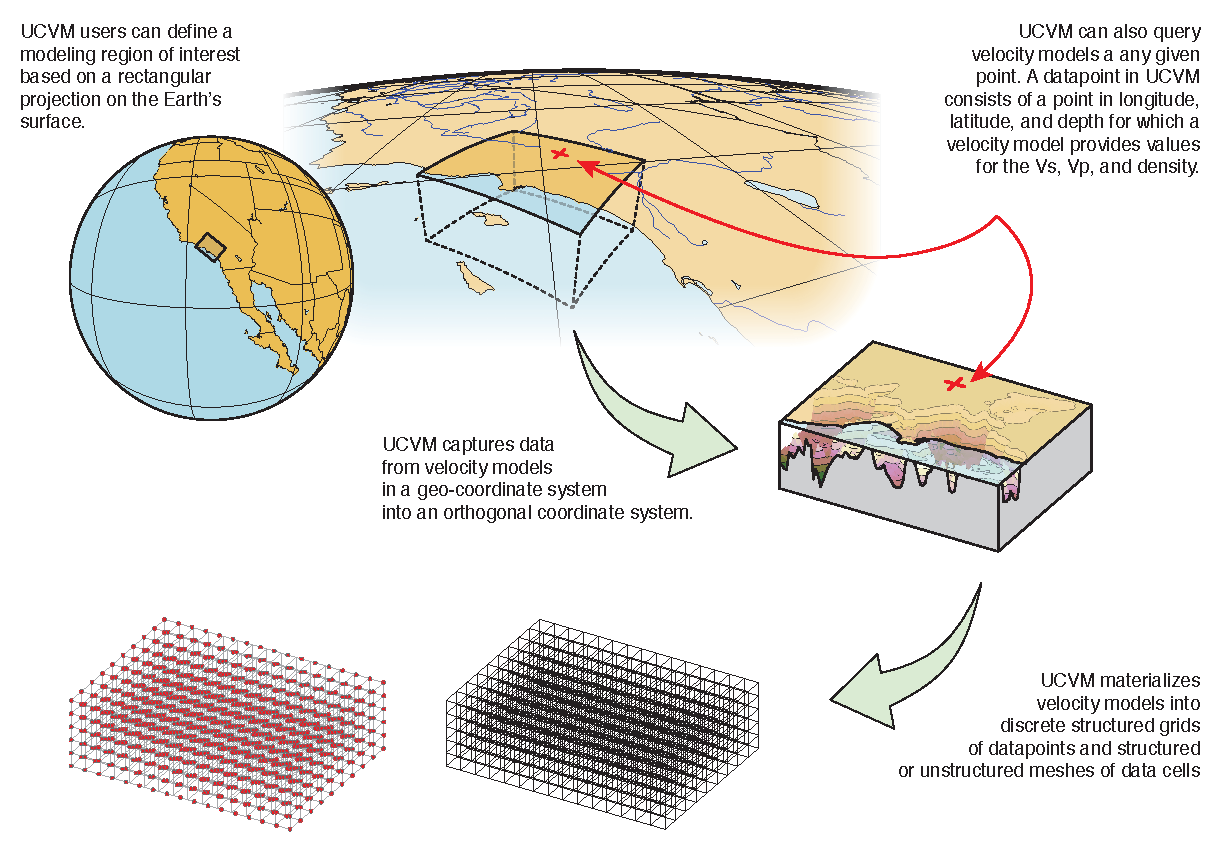
\includegraphics
		[width=0.85\textwidth]
		{figures/pdf/ucvm-model-extraction}
	\caption{High-level description of the UCVM framework functionality illustrating the selection of a region of interest for which a user can obtain datapoints using the UCVM utilities and create materialized models in the form of discrete three-dimensional grids or meshes.}
	\label{fig:framework}
\end{figure*}




\begin{figure*}[ht!]
	\centering
	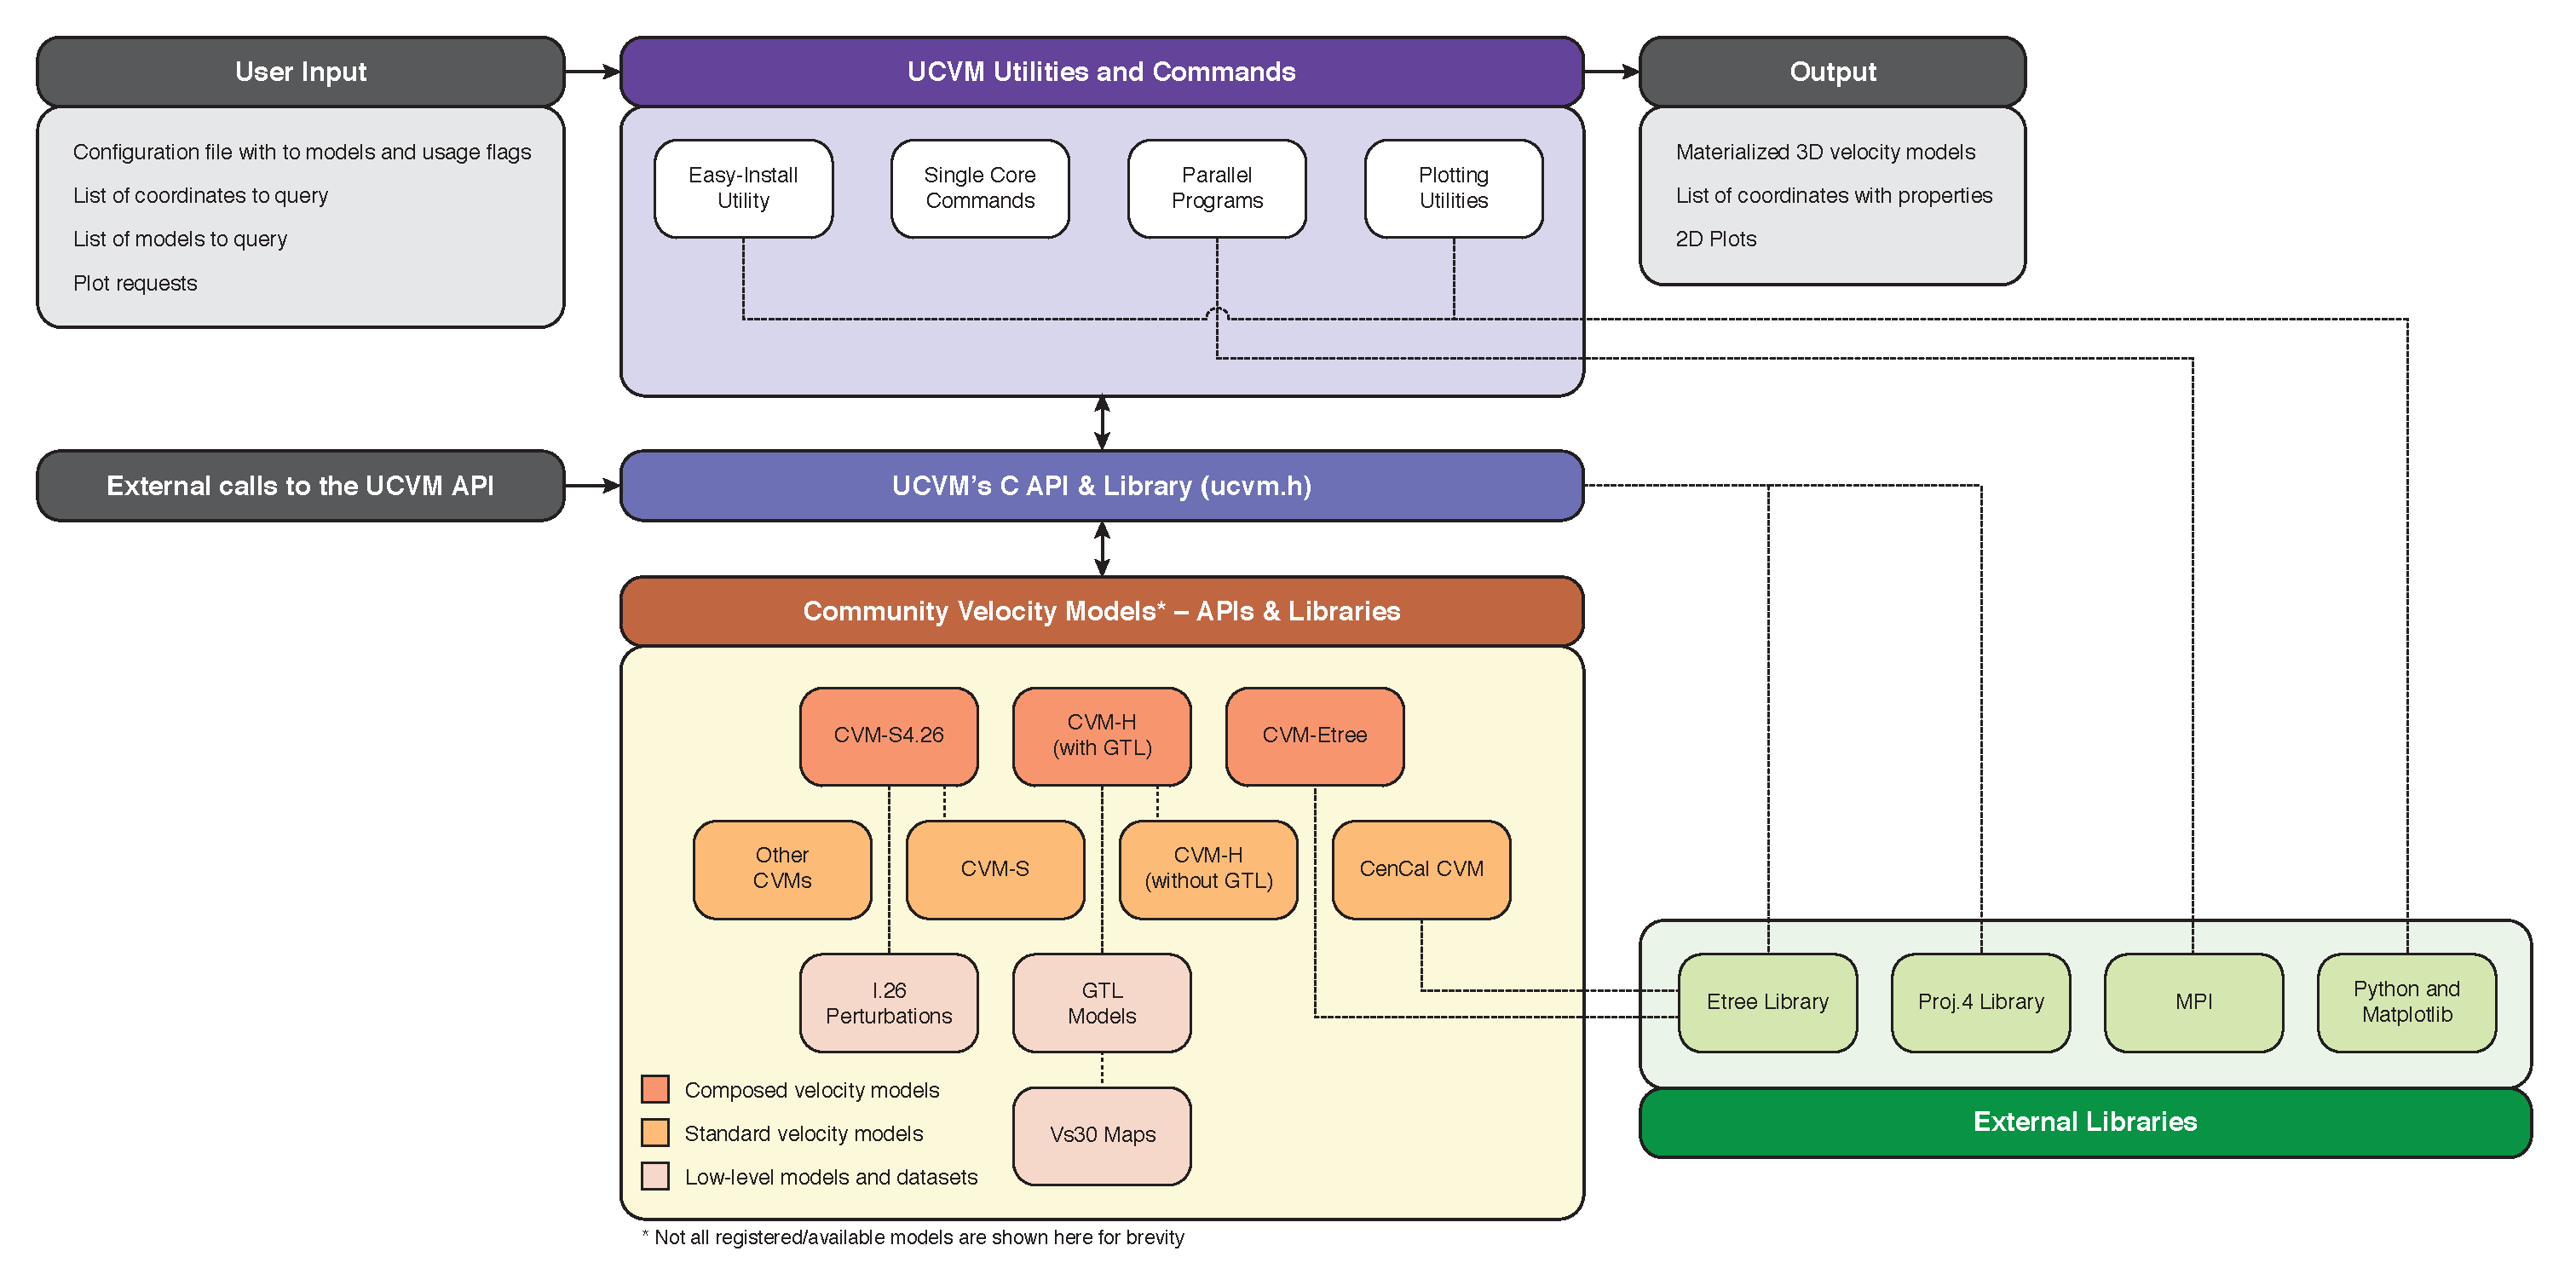
\includegraphics
		[width=\textwidth]
		{figures/pdf/ucvm-sw-architecture}
	\caption{The UCVM software architecture. Gray-colored frames indicate components at the level of user or client interaction. The upper purple-colored frame displays UCVM utilities and commands directly accessible to users, whereas the ligher purpled-colored box indicates the lower-level UCVM API and library upon which UCVM operations rest. Underlying this, are a selection of community models supported by UCVM; and to the right, in green, are the library dependencies of the UCVM framework. Here we distinguish models and datasets in four categories related to their origin or operational concept. In practice, however, UCVM treats each model or dataset independently and without any distinction.}
	\label{fig:sw.arch}
\end{figure*}



\begin{table*}
\centering
\small
\caption{Electronic addresses to UCVM on-line documentation.}
\begin{tabular}[]{ll}
\\
Description                 & URL Address                                                         \\
\hline
General Documentation       & \url{http://scec.usc.edu/scecpedia/UCVM}                            \\
General User Guide          & \url{http://scec.usc.edu/scecpedia/UCVM_User_Guide}                 \\
Latest Version (14.3) Guide & \url{http://scec.usc.edu/scecpedia/UCVM_14.3.0_User_Guide}          \\
Advanced User Guide (14.3)  & \url{http://scec.usc.edu/scecpedia/UCVM_14.3.0_Advanced_User_Guide} \\
Tutorial (14.3)             & \url{http://scec.usc.edu/scecpedia/UCVM_14.3.0_Tutorial}            \\
\hline
\end{tabular}
\label{tab:manuals}
\end{table*}


\section{The UCVM Software Framework}\label{sec:ucvm}

\subsection{Overview}

The primary functionality provided by UCVM is the ability to query a wide array of CVMs for material properties through a standardized query interface, and return material properties from the CVMs in standardized formats, independently of the particularities of each dataset or CVM. UCVM achieves this by registering datasets and velocity models into the framework. Registration of a velocity model or dataset consists of creating the appropriate API to facilitate the communication between the framework utilities and tools, and the velocity models and datasets. Once a velocity model or dataset has been registered with UCVM, a client can use the framework utilities to retrieve information from the models at any geographic point within the coverage region of the model(s). A client can be either a user (via the command-line) or a software application. The primary data type retrieved by a UCVM client for a single geographical point consists of a float triplet with the seismic velocities (\vp{} and \vs{}), and the material's density ($\rho$). At times we refer to this triple as the payload. The UCVM can then be used to produce standardized output in the form of three-dimensional (3D) volumetric datasets, two-dimensional (2D) vertical cross-sections and horizontal slices, and individual data points. This process is illustrated at a general level for the cases of 3D models in Figure \ref{fig:framework}. A client can also use other UCVM utilities for plotting and transforming models and datasets.

In order to facilitate access to the models, UCVM conceals each model's local coordinate system behind a generic querying interface. Data points are queried through this interface by geographic latitude and longitude, and a vertical $z$-coordinate. The framework allows defining the $z$-axis as either depth below the free surface (in meters, positive downward) or elevation relative to mean sea level (where zero is at sea level, positive upward and negative downward). The UCVM standardized interface allows multiple velocity models to be aggregated into a single composite model or meta-model. Composition is accomplished by tiling two or more velocity models in three dimensions according to a user-specified priority order. To support this flexible query mechanism consistently across all models, UCVM includes a high-resolution digital elevation model (DEM) and uses a cartographic projection library (Proj.4: \url{http://trac.osgeo.org/proj}). The DEM is synthesized from the U.S.~Geological Survey (USGS) National Elevation Dataset \citep{Gesch_2002_PERS, Gesch_2007_Chap} and the ETOPO1 Global Relief Model \citep{Amante_2009_Manual}. The built-in DEM enables clients to retrieve the surface elevation at any query point in addition to the default data-point payload of material properties (\vp{}, \vs{}, $\rho$).

The abstraction of native CVM interfaces under a uniform API is illustrated by Figure \ref{fig:sw.arch}. This API is written in the C language, and may be invoked directly by an application program to query any registered model as described previously. Alternatively, the framework provides a small set of predefined command-line tools to perform common operations, such as querying points, creating meshes, and producing simple graphs. As these tools are themselves defined in terms of the API, they may be leveraged as templates for creating new utilities. This layered approach to the framework design allows for future extensibility both in terms of new model support, and querying functionality.

With the exception of the Wasatch Front (Utah) CVM, the primary focus area of UCVM has been on models available for the State of California (and portions of neighboring States). However, the framework has been designed to be easily modified to cover any arbitrary region of the Earth's surface, provided adequate resolution velocity and elevation models exist. Additional details about the models available through UCVM are given in the following section on Community Velocity Models. Subsequent sections provide further information on the main UCVM features. However, due to space limitations, not all utilities and options are described in detail here. For additional in-depth information, general and advanced users should refer to the on-line manuals and documentation. Table \ref{tab:manuals} provides URL addresses linking to permanent supporting material. The last section of the paper is dedicated to simple examples and recent case applications of UCVM. 



\begin{figure*}[ht!]
	\centering
	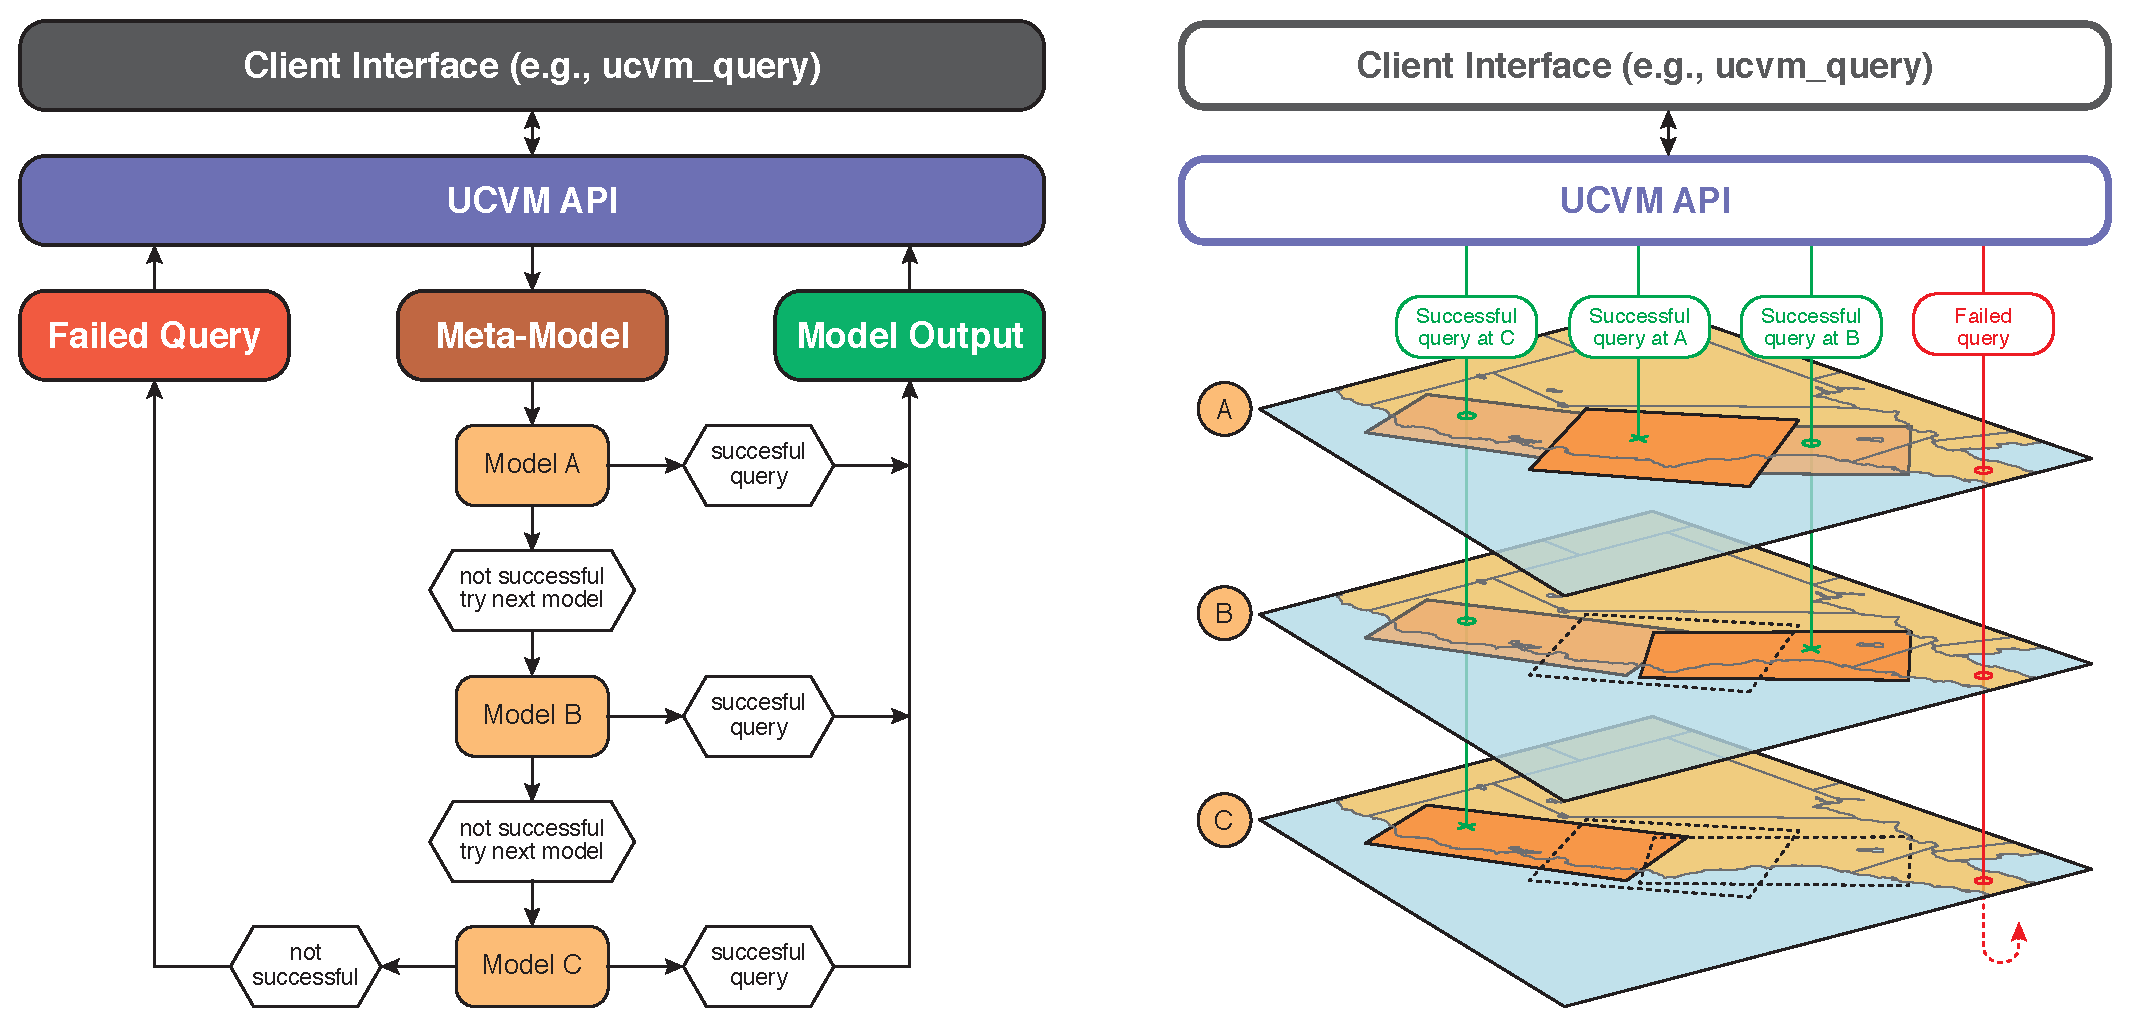
\includegraphics
		[width=0.75\textwidth]
		{figures/pdf/ucvm-query}
	\caption{UCVM querying scheme (left) and geographical illustration of the querying process (right). Information at a given geographic location is retrieved from the models registered in UCVM through a hierarchical querying scheme in which the user defines a preferred sequence of models, which are assembled internally in a meta-model. Queries to the models beneath the meta-model are carried out in the order specified by the user. Successful queried values (or failed-query results) are handled by the UCVM API wich is accessible to the user/client through a predefined interface such as the program \texttt{ucvm\_query}.}
	\label{fig:tiling}
\end{figure*}


\subsection{Querying Material Properties}
\label{sec:querying}

UCVM provides two methods for querying models. The first method is programmatically, directly through the provided C language API. The second is via the command-line program \texttt{ucvm\_query}. Both methods query the underlying models in the same manner; the \texttt{ucvm\_query} program is merely a simplified front-end layered upon the API.

The query process begins with the identification of one or more CVMs as the source of material properties. In this respect, the framework distinguishes between geotechnical layers and standard crustal models, allowing the user to make selections for both. As illustrated in Figure \ref{fig:tiling}, the set of standard crustal models is tiled in three dimensions to form a meta-model. The same operation is performed on the GTLs to define a meta-GTL. The interface between the meta-GTL and meta-model is then smoothed using an interpolation function (linear interpolation in the simplest case) along a user-defined interpolation zone parallel to the z-axis. Note that when two or more models overlap in three dimensional space, the model listed first within the tiling order will satisfy requests within that overlapping zone.

Once the models have been tiled in this manner, the API or program accepts one or more input query points from the user. For every point, the framework queries each component model of the two meta models, until either a valid set of velocities and density are returned, or all component models have been queried and the request was unsatisfied. Thus, for points that fall within the interpolation zone, two sets of material properties may be generated---one for each meta model. These two sets of material properties are then combined using the interpolation function. As the native query interfaces of available CVMs accept query points in a wide array of formats (e.g., geographic coordinates versus UTM-11 map coordinates, or depth versus elevation for the vertical component), UCVM may perform a coordinate transformation to convert its input format of decimal (latitude, longitude, depth/elevation) tuples to the local coordinate system of the component model being queried. This is accomplished transparently by utilizing the standard projection library Proj.4 \citep{Evenden_2003_Manual}.

In the case of the API, the result of a successful query is a data-structure containing the velocities \vp{} and \vs{}, and the density $\rho$ at the point of interest, along with the elevation in meters and $V_{S30}$ value of the corresponding point on the free-surface. This data-structure also includes an indicator of which velocity model within the meta-model ultimately satisfied the request. For those points which fall within the interpolation zone between the meta-GTL and meta-model, the framework additionally identifies the material properties reported by the meta-GTL and the meta-model, as well as the component models from which they were extracted. For the \texttt{ucvm\_query} program, this same information is formulated in tabular format and printed to the screen.

This tiling mechanism mostly allows one to complement missing information in one model with that of other overlapping or underlying models. In the future, the UCVM tiling feature could be used as tool for combining multiple regional velocity models. The platform, however, does not presently provide built-in functionalities to do so beyond the described tiling mechanism. The reason being that consistency problems arise when velocity models overlap in three-dimensional space. That is, tiling two overlapping models that are not compatible has the potential of creating interfaces with unnatural contrasts. These artifacts are undesirable for earthquake simulation applications because they can cause unexpected wave reflections or refractions. There are two approaches one can take to remedy this problem. The simplest approach is to define a UCVM patch model to trilinearly interpolate the material properties within a certain geographic region. This patch model may be tiled along with the overlapping traditional velocity models to produce a smoothed meta-model. However, this numerical smoothing approach may not reflect the physical structures of the Earth's surface. The second approach is to utilize UCVM to query all models within the overlap zone individually, and then manually combine the results with a user-defined interpolation function. We expect that future tomographic inversions of larger regions will allow us to integrate better models or algorithms to handle this situation.


\section{Community Velocity Models}
\label{sec:cvms}

The UCVM framework supports different seismic velocity models. 

(temp material)

Community velocity models vary widely in their area of coverage, depth extent, and resolution. UCVM is flexible in its support for such variability. However, in order to better accommodate high frequency ground motion simulations, it categorizes models into two general groups: crustal models, and geotechnical layers (GTLs). Crustal models provide subsurface seismic wave velocities associated with basin, crust, and mantle structures. These models may potentially extend to many tens of kilometers below the Earth's surface yet do so at coarse resolutions (TODO: cite CVM-H, CVM-S). Geotechical layers, in contrast, provide velocities for only the near-surface (typically a few hundred meters) at very high resolution (TODO: cite Ely Vs30 GTL). Ground motion simulations, in particular, rely on high-resolution near-surface velocities and therefore a GTL serves to supplement the coarser data provided by crustal models.

TODO: Interpolation of GTL with Crustal

%\textit{
%\color{blue}
%This section will present how CVMs work and the various CVMs available to the community today. It will basically explain that CVMs provide the triplets of Vs, Vp and density, and, as an example, we can expand on a description of CVM-S and CVM-H, including their variations CVM-SI and CVM-H+GTL.
%}




\section{Community Velocity Models}
\label{sec:cvms}

The UCVM framework supports different seismic velocity models. 

(temp material)

Community velocity models vary widely in their area of coverage, depth extent, and resolution. UCVM is flexible in its support for such variability. However, in order to better accommodate high frequency ground motion simulations, it categorizes models into two general groups: crustal models, and geotechnical layers (GTLs). Crustal models provide subsurface seismic wave velocities associated with basin, crust, and mantle structures. These models may potentially extend to many tens of kilometers below the Earth's surface yet do so at coarse resolutions (TODO: cite CVM-H, CVM-S). Geotechical layers, in contrast, provide velocities for only the near-surface (typically a few hundred meters) at very high resolution (TODO: cite Ely Vs30 GTL). Ground motion simulations, in particular, rely on high-resolution near-surface velocities and therefore a GTL serves to supplement the coarser data provided by crustal models.

TODO: Interpolation of GTL with Crustal

%\textit{
%\color{blue}
%This section will present how CVMs work and the various CVMs available to the community today. It will basically explain that CVMs provide the triplets of Vs, Vp and density, and, as an example, we can expand on a description of CVM-S and CVM-H, including their variations CVM-SI and CVM-H+GTL.
%}



\section{Download and Installation}
\label{sec:installation}

The latest version of the UCVM platform is available at:
%
\url{http://hypocenter.usc.edu/research/ucvm/14.3.0/ucvm-14.3.0.tar.gz}. 
\textcolor{red}{We must use a non-versioned URL that always points to the latest version.}
%
After successfully downloading this package, the user can follow one of two possible options: the \textit{easy method} or the \textit{custom method}. The easy method uses a Python wrapper to facilitate the installation process that prompts the user about installation paths and default models to be enabled. Figure \ref{fig:instaeasy} shows the sequence of terminal commands used during the easy installation process in a Linux workstation.


\begin{figure}[th]
\begin{lstlisting}[
	frame=single,
	basewidth={0.45em,0.4em},
	backgroundcolor=\color{mylistingbkgd},
	basicstyle=\ttfamily\footnotesize,breaklines=true,
	linewidth=0.98\columnwidth,xleftmargin=0.07\columnwidth,
	numbers=left,numberblanklines=true,numberstyle=\scriptsize\color{mylistingnclr}]
> tar zxvf ucvm-14.3.0.tar.gz
> cd ./UCVM
> ./ucvm_setup.py
  It looks like you are installing UCVM for the first time.
  Where would you like UCVM to be installed?
  Enter path or blank to use default: 

  <user path entry>

  Would you like to download and install CVM-S4?
  Enter yes or no: 

  <yes,no>

  [...]
\end{lstlisting}
\caption{Easy installation procedure. Shell commands are indicated by the symbol \textgreater. \textcolor{red}{This example needs to be completed with a full installation sequence.}}
\label{fig:instaeasy}
\end{figure}

Alternatively, one can also customize the installation by directly invoking the underlying Automake \emph{configure} script. An example situation is the case when a user wishes to install a version of a CVM other than the latest supported (regression to a prior CVM release). In this case, the user must pre-install the CVMs and library dependencies themselves. When installing UCVM manually, three flags need to be provided for each model to be properly configured, namely the paths to the model data files, API library, and API include files. Similarly, the Proj4 and Euclide etree libraries must be specified with the paths to their library and include files. 

\textcolor{green}{Refer reader to the user guide as this outside scope.}

\textcolor{green}{Commented out last paragraph and fig 3 as it is too detailed.}
%As an example, Figure \ref{fig:instadvanced} shows the sequence of commands an advanced user would need to manually install UCVM in a Cray supercomputer system with default PGI compilers with static build and IO buffering, enabling the Proj4 and Etree libraries and the model CVM-S. Note that UCVM requires GNU GCC compiler 4.3+; therefore, in the example in Figure \ref{fig:instadvanced}, the user needs to switch to the GNU compilers. When installing UCVM manually, three flags need to be provided for each model to be properly configured, namely a \texttt{lib-path}, a \texttt{model-path}, and an \texttt{include-path}. Similarly, each library needs a \texttt{lib-path} and an \texttt{include-path}. The last command in the example in Figure \ref{fig:instadvanced}, \texttt{make check} will test the installation to make sure that UCVM was deployed correctly. 


%
\begin{figure}[ht!]
\centering
\begin{lstlisting}[
	frame=single,
	basewidth={0.45em,0.4em},
	backgroundcolor=\color{mylistingbkgd},
	basicstyle=\ttfamily\footnotesize,breaklines=true,
	linewidth=0.98\columnwidth,xleftmargin=0.07\columnwidth,
	numbers=left,numberblanklines=true,numberstyle=\scriptsize\color{mylistingnclr}]
> module swap PrgEnv-pgi PrgEnv-gnu
> module load iobuf
  [...]
> UCVM_DIR=<user defined path>
> UCVM_VERSION=14.3.0
> ROOT_URL=http://hypocenter.usc.edu/research/ucvm
> LIBS_URL=$ROOT_URL/$UCVM_VERSION/libraries
> MODELS_URL=$ROOT_URL/$UCVM_VERSION/models
  [...]
> cd $UCVM_DIR
> wget $LIBS_URL/proj-4.8.0.tar.gz
> wget $LIBS_URL/euclid3-1.3.tar.gz
> wget $MODELS_URL/cvms4.tar.gz
  [...]
> tar xzvf proj-4.8.0.tar.gz
> cd proj-4.8.0
> ./configure --prefix=$UCVM_DIR/lib/proj-4 --with-jni=no
> make
> make install
  [...]
> cd $UCVM_DIR
> tar xvzf euclid3-1.3.tar.gz
> cd euclid3-1.3
> ./configure --prefix=$UCVM_DIR/lib/euclid3
> make; make install
  [...]
> cd $UCVM_DIR
> tar xzvf cvms4.tar.gz
> cd CVM-S
> ./configure --prefix=$UCVM_DIR/model/cvms4
> make
> make install
  [...]
> cd $UCVM_DIR
> tar xzvf ucvm-14.3.0.tar.gz
> cd UCVM
> ./configure \
  --prefix=$UCVM_DIR \
  --enable-iobuf \
  --enable-static \
  --with-etree-include-path=$UCVM_DIR/lib/euclid3/include \
  --with-etree-lib-path=$UCVM_DIR/lib/euclid3/lib \
  --with-proj4-include-path=$UCVM_DIR/lib/proj4/include \
  --with-proj4-lib-path=$UCVM_DIR/lib/proj4/lib \
  --enable-model-cvms \
  --with-cvms-lib-path=$UCVM_DIR/model/cvms4/lib \
  --with-cvms-model-path=$UCVM_DIR/model/cvms4/src \
  --with-cvms-include-path=$UCVM_DIR/model/cvms4/src
> make
> make install
> make check
  [...]
\end{lstlisting}
\caption{Advanced installation procedure showing the commands a user will follow when working on a Cray supercomputer system with default PGI compilers and Lustre filesystem. Note that UCVM requires GNU GCC compilers, version 4.3+. This particular set of instructions installs the model CVM-S (version 4) with the Proj and Etree libraries using static build and enabling IO-buffering. Shell commands are indicated by the symbol \textgreater. \textcolor{red}{This example needs to be checked.}}
\label{fig:instadvanced}
\end{figure}






\section{Features}

The UCVM platform offers an API and a set of programs, many of which can be used either in a single processor context or in parallel. This section details the most relevant of these programs, categorized by the broad feature they are intended to support. The discussion will focus largely on how the single processor programs operate. Those features that have additional support for parallel computing will be noted, and any operational differences between the single core and parallel implementations shall be described.

The single-core commands can be run in any system where the platform has been successfully installed. The parallel commands, however, require a system where the standard Message Passing Interface (MPI) library and compilers are available. Single-core commands are useful to most users interested in exploring the properties of the regions covered by the models supported by the platform. On the other hand, advanced users needing to build large-scale (regional) materialized velocity models for earthquake modeling and simulation are the more likely to use the MPI commands. 

%\textcolor{green}{For each utility, we should implicitly answer four questions as a narrative. 1) What problem is this utility trying to solve? 2) How does this utility solve the problem? 3) What information does the user need to provide? 4) What does the utility output? For the input description, rather than providing a configuration file, I would use a table with the relevant parameters to the problem and a description of each (ignoring simple things like output file paths, number of processors, etc).}


\begin{figure*}[ht!]
	\centering
	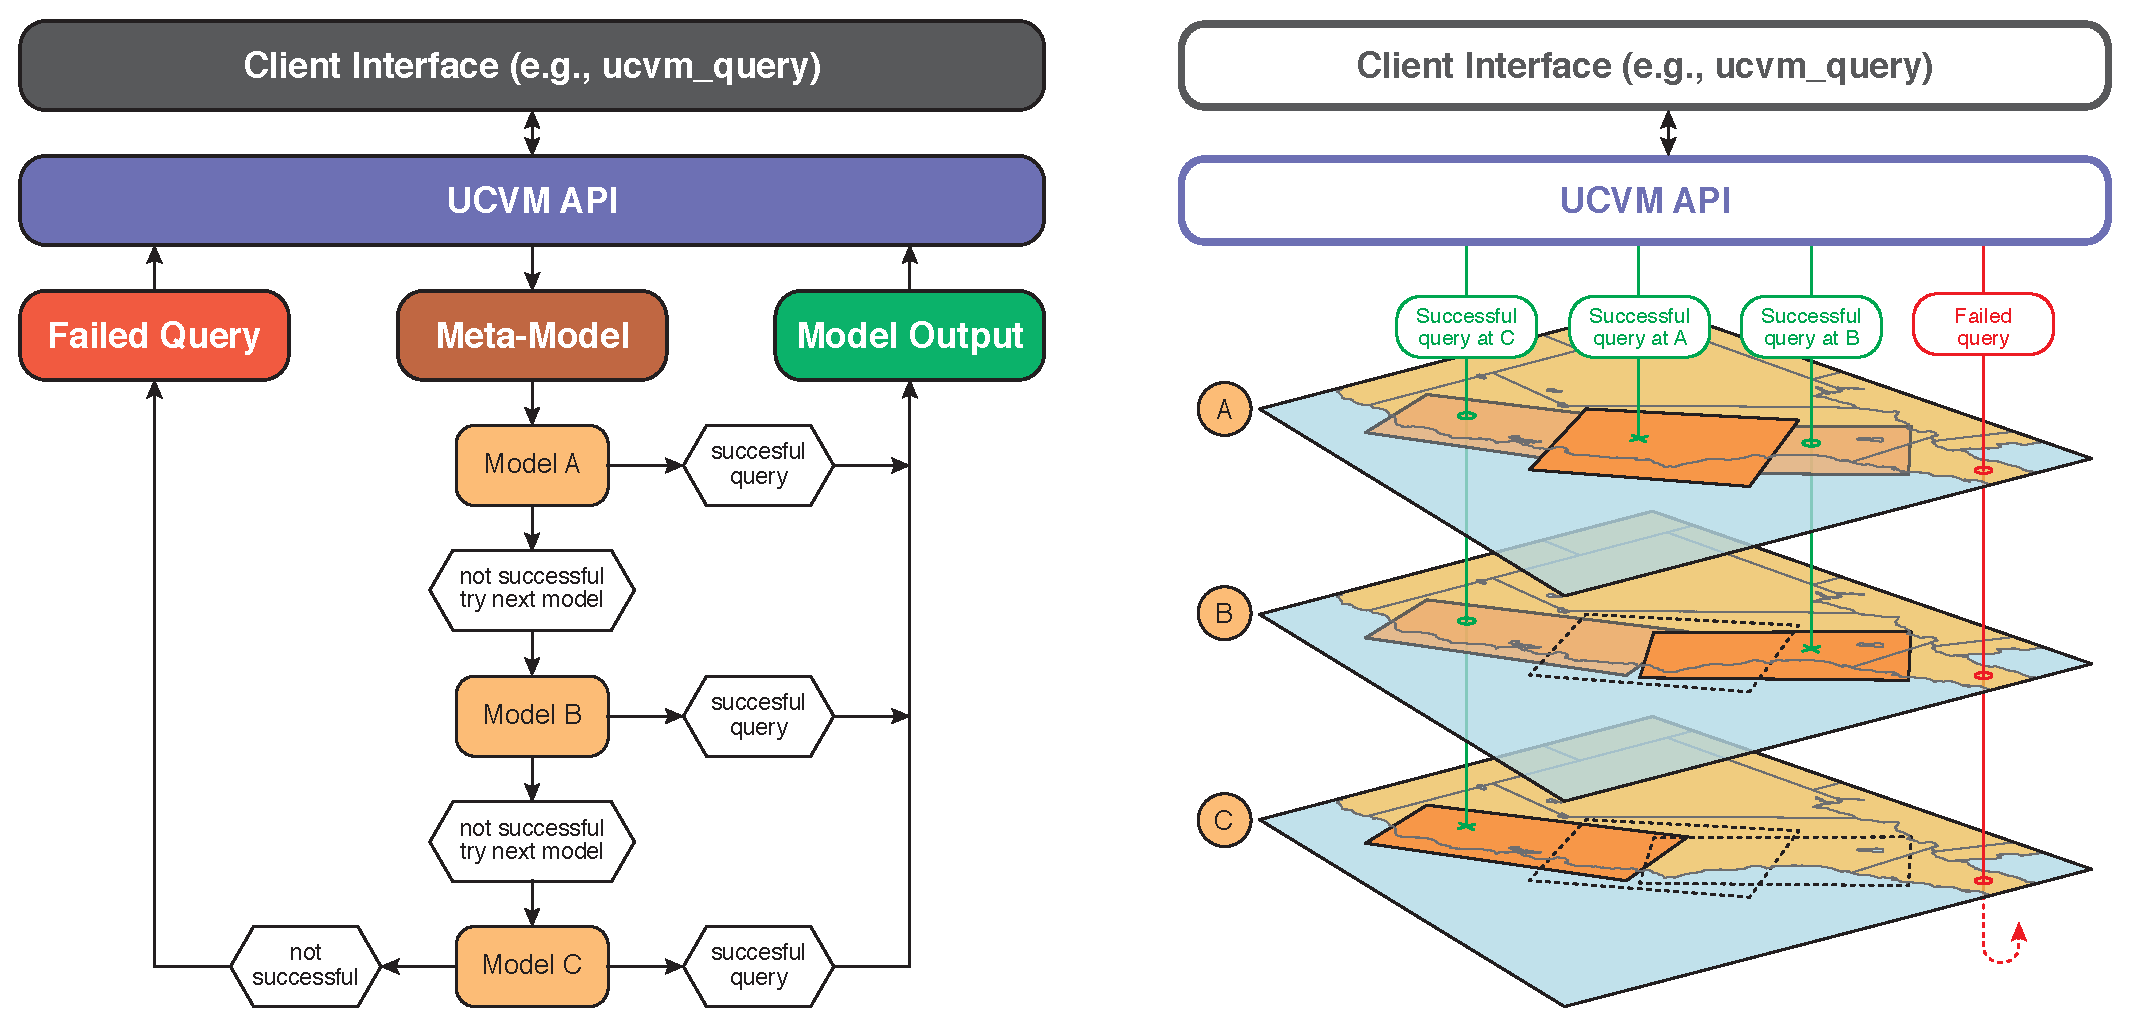
\includegraphics
		[width=0.75\textwidth]
		{figures/pdf/ucvm-query}
	\caption{UCVM querying scheme (left) and geographical illustration of the querying process (right). Information at a given geographic location is retrieved from the models registered in UCVM through a hierarchical querying scheme in which the user defines a preferred sequence of models, which are assembled internally in a meta-model. Queries to the models beneath the meta-model are carried out in the order specified by the user. Successful queried values (or failed-query results) are handled by the UCVM API wich is accessible to the user/client through a predefined interface such as the program \texttt{ucvm\_query}.}
	\label{fig:tiling}
\end{figure*}


\subsection{Querying Material Properties}

UCVM provides two methods for querying models. The first method is programmatically, directly through the provided C language API. The second is via the command-line program \texttt{ucvm\_query}. Both methods query the underying models in the same manner; the \texttt{ucvm\_query} program is merely a simplified front-end layered upon the API.

The query process begins with the identification of one or more CVMs as the source of material properties. In this respect, the framework distinguishes between geo-technical layers and standard crustal models, allowing the user to make selections for both. As illustrated in Figure \ref{fig:tiling}, the set of standard crustal models is tiled in three dimensions to form a meta-model. The same operation is performed on the GTLs to define a meta-GTL. The interface between the meta-GTL and meta-model is then smoothed using an interpolation function (linear interpolation in the simplest case) along a user-defined interpolation zone parallel to the z-axis. Note that when two or more models overlap in three dimensional space, the model listed first within the tiling order will satisfy requests within that overlapping zone.

Once the models have been tiled in this manner, the API or program accepts one or more input query points from the user. For every point, the framework queries each component model of the two meta models, until either a valid set of velocities and density are returned, or all component models have been queried and the request was unsatisfied. Thus, for points that fall within the interpolation zone, two sets of material properties may be generated - one each for each meta model. These two sets of material properties are then combined using the interpolation function. As the native query interfaces of available CVMs accept query points in a wide array of formats (geographic coordinates versus UTM-11 map coordinates, or depth versus elevation for the vertical component, for example), UCVM may perform a coordinate transformation to convert its input format of decimal (latitude, longitude, depth/elevation) tuples to the local coordinate system of the component model being queried. This is accomplished transparently by utilizing the standard projection library Proj.4 (NOTE: cite Proj.4).

In the case of the API, the result of a successful query is a data-structure containing the velocities $V_{p}$ and $V{s}$, and the density $\rho$ at the point of interest, along with the elevation in meters and $V_{S30}$ of the corresponding point on the free-surface, and an indication of which velocity model within the meta-model ultimately satisfied the request. For those points which fall within the interpolation zone between the meta-GTL and meta-model, the framework additionally identifies the material properties reported by the meta-GTL and meta-model, as well as the component models from which they were extracted. For the \texttt{ucvm\_query} program, this same information is formulated in tabular format and printed to the screen.

This tiling mechanism can be a powerful feature for combining multiple regional velocity models, but a problem arises when velocity models overlap in three-dimensional space. Simply tiling two overlapping models will create a three-dimensional interface that may contain sharp contrasts in either velocities or density. This artifact is undesirable for earthquake simulation applications as it can cause reflections in wavefronts. There are two approaches to remedy this problem. The simplest approach is to define a UCVM patch model to trilinearly interpolate the material properties within arbitrary cuboid geographic region. This patch model may be tiled along with the overlapping traditional velocity models to produce a smoothed meta-model. However, this numerical smoothing approach does not reflect the physical structures of the Earth's surface. The second approach is to utilize UCVM to query all models within the overlap zone individually, and then manually combine the results with a user-defined interpolation function. 


% ---------------------------------------------------------------------------------------------
% TEMP FIGURE: Needs to be completed and improved in Illustrator and moved to final PDF dir.
\begin{figure*}[ht!]
	\centering
%	\includegraphics
%		[width=0.75\textwidth]
%		{figures/raw-pdf/covered-areas}
	\fbox{\begin{minipage}{\textwidth}\textcolor{red}{PENDING}\vspace{2in}\end{minipage}}
	\caption{Construction of a mesh with the program ucvm2mesh.}
	\label{fig:meshing}
\end{figure*}
% ---------------------------------------------------------------------------------------------


\subsection{Creating Structured 3D Meshes}

The framework may be utilized to generate a structured uniform mesh in a format consistent with those used by the AWP-ODC and SORD (NOTE: need to confirm if SORD still uses this format) simulation codes with the program \texttt{ucvm2mesh}.

Construction of mesh proceeds as shown in Figure \ref{fig:meshing}. The user specifies a two-dimensional map projection (such as UTM-11), a latitude and longitude geographic anchor point, mesh cell dimensions ($nx$, $ny$, $nz$) along the x,y and z axis (where x-y is in the plane of the projection and z is vertical), step size $dx$ in meters, and rotation angle within the map projection. Additionally, the user provides a list of CVMs to query, and these models are tiled in the same manner as was described in the previous section.

The program \texttt{ucvm2mesh} projects the geographic coordinates of the Earth's surface into the map projection, placing the origin of the mesh as the anchor point and discretizing the volume according to the provided dimensions and step size. For each point in the projected volume, \texttt{ucvm2mesh} determines the analous geographic point in terms of (latitude, longitude, depth) and queries the underlying CVMs for material properties. These material properties are then assigned to the mesh point.

Four binary mesh formats are supported: IJK-12, IJK-20, IJK-32, and SORD. The first three formats are mesh variants used by AWP-ODC (NOTE: cite) and the last format is used by SORD (NOTE: cite and check if still true). For IJK-12 formatted meshes, the output is a binary file consisting of a list of nx*ny*nz tuples. Each tuple contains three single precision floating point values $(V_p. V_s, \rho)$, representing the material properties for a point in the mesh, with the mesh coordinates given implicitly by the position of the tuple in the list. The tuples are arranged in x-y-z order. 

Similarly, the IJK-20 format adds the seismological parameters $\mu$ and quality factor $Q$ so that each tuple contains $(V_p. V_s, \rho, mu, Q)$ (NOTE: confirm and explain mu and Q), while the IJK-32 format extends IJK-20 further by adding the three four-byte integers $(i,j,k)$ to each tuple, representing the index coordinate of the grid cell within the mesh. Thus, in this latter case, each tuple contains $(i, j, k, V_p. V_s, \rho, mu, Q)$.

(NOTE: Explain SORD format)

(NOTE: Note ucvm2mesh-mpi exists, I don't think there are any operational differences)


\begin{figure*}[ht!]
	\centering
	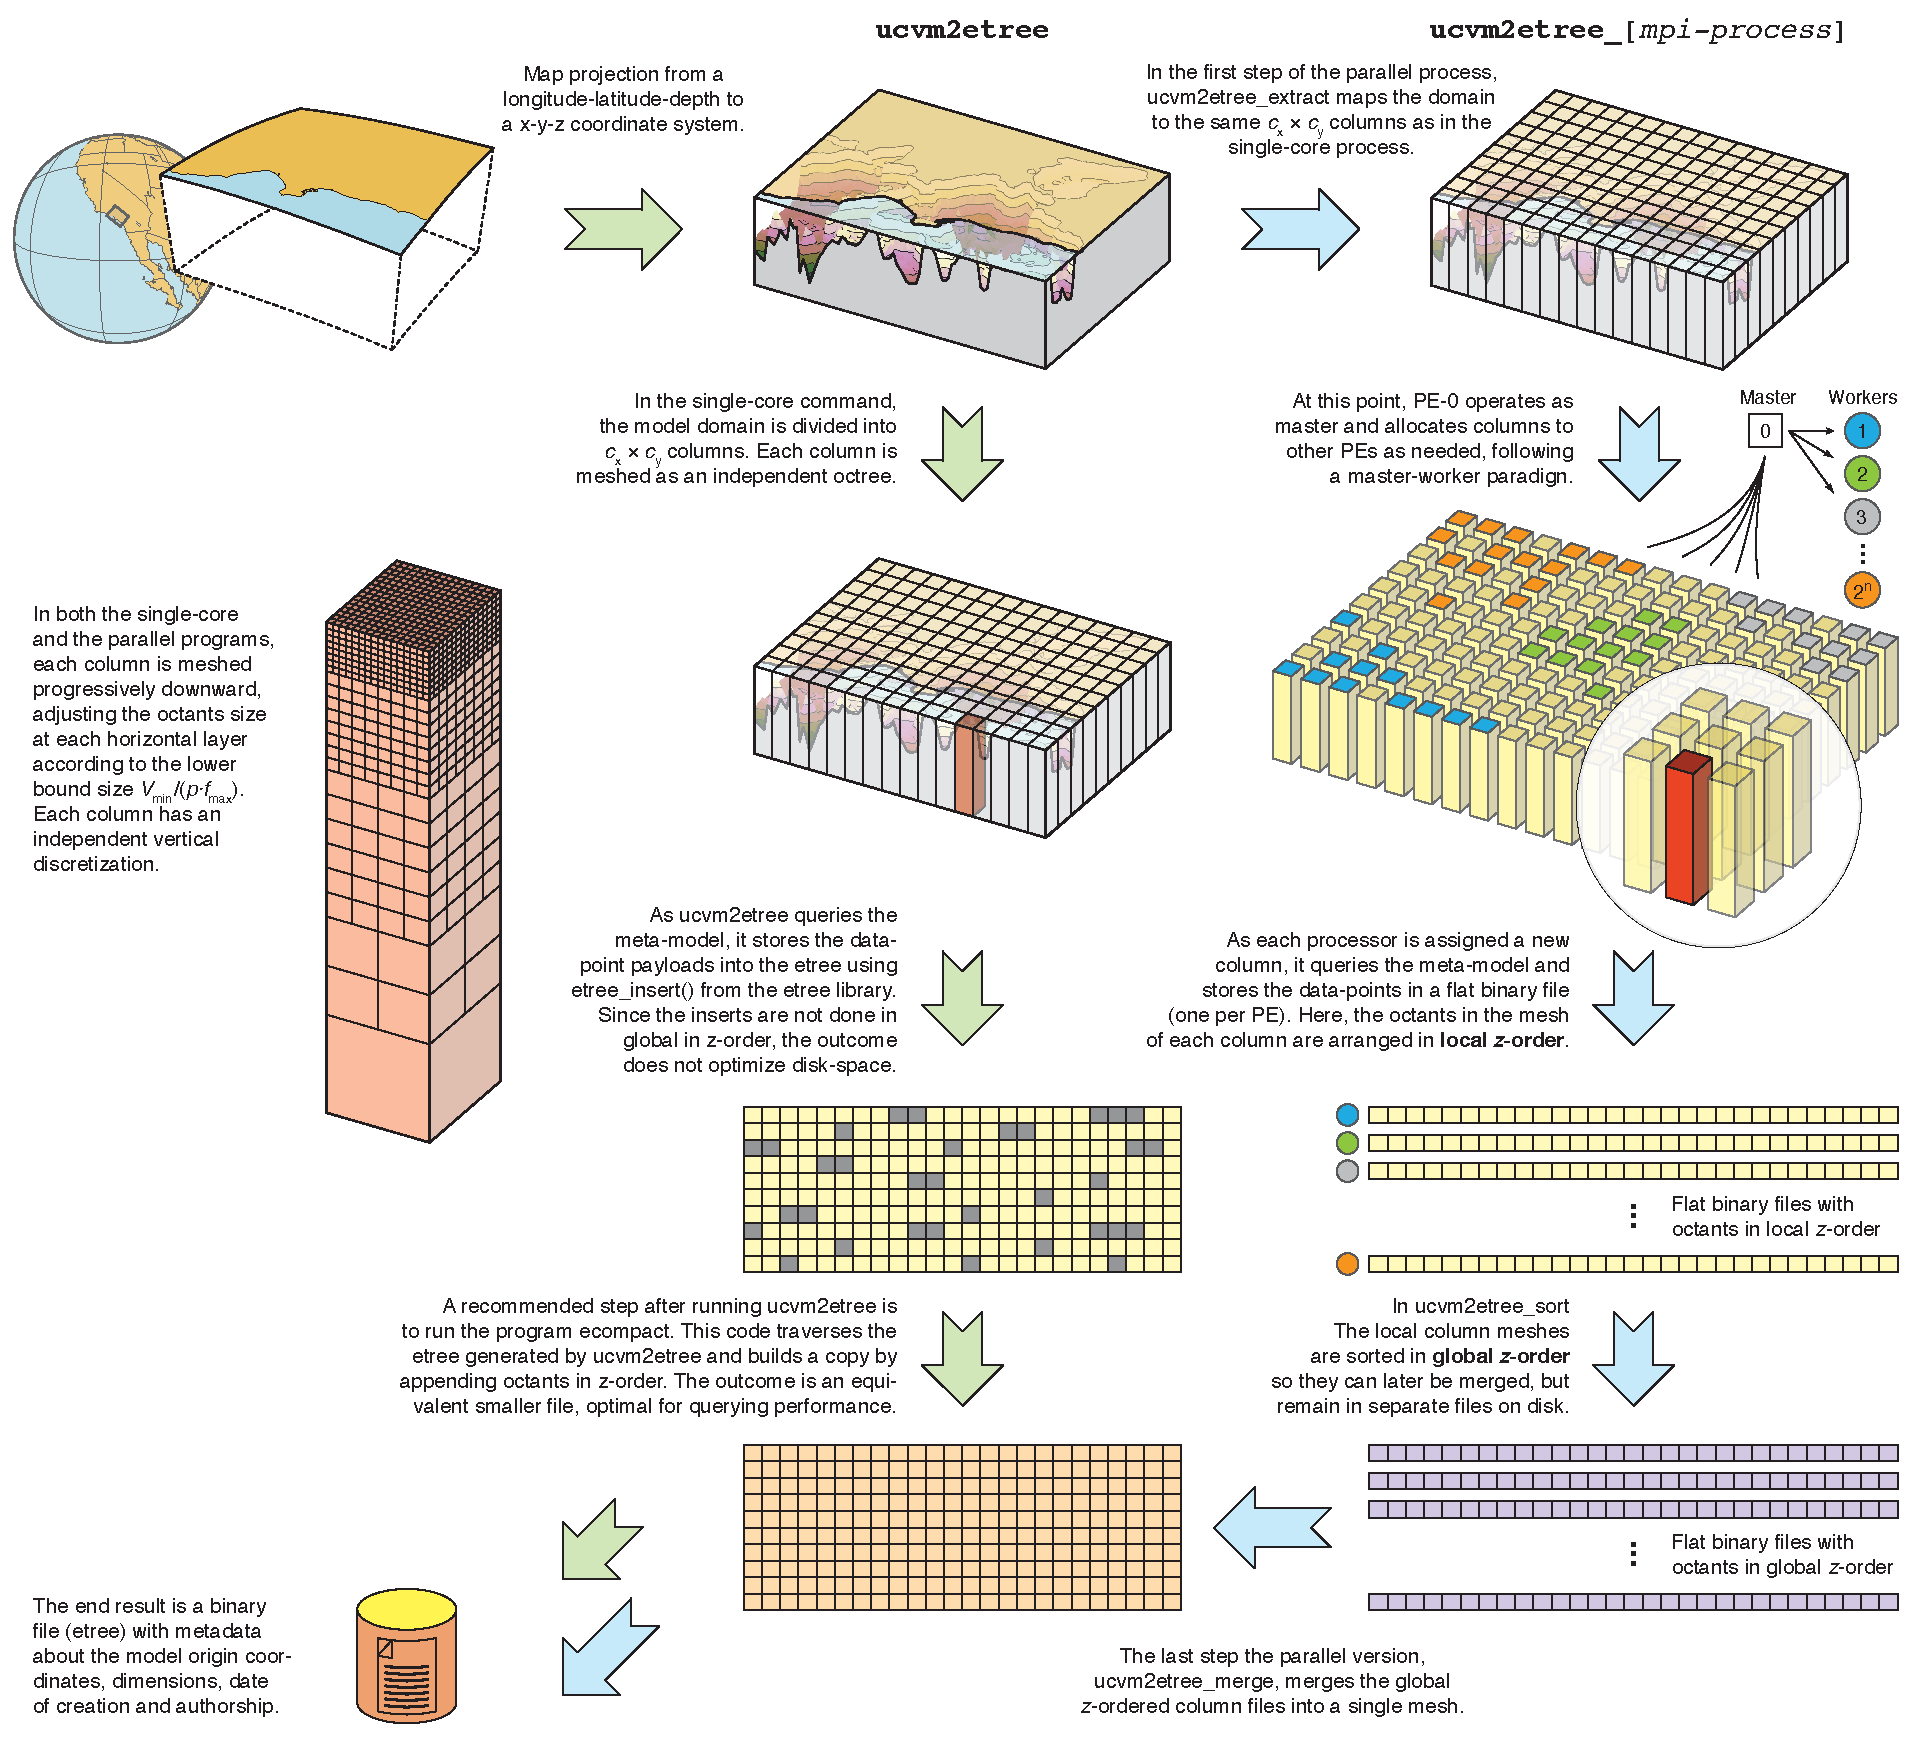
\includegraphics
		[width=\textwidth]
		{figures/pdf/ucvm-to-etree}
	\caption{Construction of an semi-unstructured mesh in the Etree database format using the program \texttt{ucvm2etree} (green arrows); and its MPI equivalent process controlled by the programs \texttt{ucvm2etree\_extract}, \texttt{ucvm2etree\_sort} and \texttt{ucvm2etree\_merge} (blue arrows). Note that in contrast to the structured grid construction process, here the information payload (\vs{}, \vp{}, and $\rho$) is associated with the octants in the octree structure and not with a point. In other words, the querying and assignment process mapps the information queried at the center of each octant to the whole volume enclosed by the octant.}
	\label{fig:etrees}
\end{figure*}
% ---------------------------------------------------------------------------------------------


\subsection{Creating Etree Databases}

TBD, reference Figure \ref{fig:etrees}

\subsection{Miscellaneous Features}

TBD

\subsubsection{Querying Iso-surfaces}

TBD 
%\texttt{basin\_query} and \texttt{basin\_query-mpi}


\subsubsection{Small-scale Heterogeneities}

The last decade has seem a tremendous growth on high performance computing and applications dedicated to earthquake ground motion simulations which is leading the charge toward performing deterministic simulations at high frequencies of engineering interest (\fmax{} 0--10 Hz). With increasing simulation frequencies, seismic velocity models must not only be accurate representations of a region's crustal structure at the geologic scale and represent the geotechnical characteristics of basins and deposits, but should also provide for the adequate representation of the scattering characteristics of the typical heterogeneities observed in geomaterials. To this end, UCVM implements an algorithm generates models that incorporate small-scale heterogeneities to any underlying velocity model. The command \texttt{ssh\_generate} generates a binary float file of heterogeneities on a regular grid space with a normalized amplitude. Then, the command \texttt{ssh\_merge} adds the heterogeneities multiplied by some scaling factor to the model. The introduction of the heterogeneities is actually done by applying the scaled perturbation to the slowness of the underlying mesh velocities, and then converted back to the seismic velocity. The following example generates and merges a set of small scale heterogeneities to ... \textcolor{red}{describe example}.

\subsubsection{Etree Optimization}

TBD \texttt{ecoalasce}, etc

\subsubsection{Visualization}

%\textcolor{green}{I would collapse all of these subsections into one, basically stating that there is a limited plotting facility included with UCVM that supports cross-sections, horizontal slice, $V_{s30}$ maps, and iso-surfaces. And then a short description of each. I think the placeholder plots (Fig 6 marked as pending) are OK and we can show some/all of them. We can provide a detailed plotting use case in the Examples section. They are all fairly similar in that they are Python scripts that utilize the matplotlib Python module (I presume, if these scripts are based on others I developed in a separate code repository) for the actual plotting, while querying for material properties with either ucvm\_query or basin\_query.}

%\textcolor{green}{Also, with the inclusion of these scripts, does UCVM now depend on Python with matplotlib? If so, we should add that to the list of dependencies in the framework section as well as list it on the wiki. Or are these scripts optional?}

This section briefly describes a collection of utilities provided with the UCVM platform. These utilities are written in Python scripts that operate as wrappers around the basic single-core commands explained above, and work to produce specific output data commonly used for plotting. Because of brevity, we cannot fully describe here all the options and parameters that each of these commands can take as input and will only illustrate their operability. Additional details can be found at the UCVM User Guide (see Table \ref{tab:manuals}).


\section{Utilities}
\label{sec:utilities}

The UCVM platform 

%\subsection{Querying}
%
%\subsection{Gridding and Meshing}
%
%\subsection{UCVM and the Etree Library}
%
%\subsection{New DEMs and Vs30 Maps}


%
%\section{Parallel Utilities}
%
%\section{Application Programming Interface}
%
%
%\section{Computational Performance}
%\label{sec:conclusions}
%
%\textit{
%\color{blue}
%It would be desirable to do some experiments in terms of performance, especially for the parallel applications utilities in UCVM. With some examples of how long the same thing would take if doing it differently. We will need to discuss this.
%}
%
%\section{Recent Case Applications}
%\label{sec:conclusions}
%
%\textit{
%\color{blue}
%This section will be dedicated to show case applications. Some ideas for potential subsections follow.
%}
%
%\subsection{Visualization and Model Comparisons}
%
%\subsection{Chino Hills Simulation Series}
%
%\subsection{CyberShake}
%
%\section{Summary and Conclusions}
%\label{sec:conclusions}
%
%\textit{
%\color{blue}
%A couple of paragraphs with a summary of what is shown in the paper and a few key conclusions about the impact that we expect UCVM has already have and will have on earthquake research.
%}

